\section{Applications in Observer Geometry}
\label{sec:application}

\subsection{A terrestrial viewing window}

For the terrestrial application, we determine when a target exceeds
$30^\circ$ altitude during 2025 January 1 UTC at a site with longitude $1.5^\circ$ east, geodetic latitude $42^\circ$
north and zero ellipsoidal height. The prescribed direction has right ascension
$120^\circ$ and declination $20^\circ$ in the true equator and equinox of date.
It defines a reproducible pointing scenario with fixed angular coordinates.

The calculation constructs a UTC epoch, converts it to TT and calls
\texttt{to\_horizontal\_precise} with a separately typed UT1 epoch and the
site. We prescribe $\mathrm{UT1}-\mathrm{UTC}=0$ for this example and sample
\ViewingSampleCount{} epochs at five-minute spacing, including both day
endpoints. Selection above the threshold produces \ViewingSelectedCount{}
samples spanning \ViewingSpans{} UTC.
Figure~\ref{fig:viewing-window} displays the complete grid.
These are selected sample spans; threshold crossings lie between adjacent
five-minute samples and are not root-refined rise or set times.

The independent reduction combines ERFA \texttt{gst06a} and \texttt{hd2ae}
with the same inputs. The maximum altitude difference is below
$\AltitudeBound$ degrees. Site geometry, angular units, frame and time scales
remain explicit throughout the selection, illustrating how a simple planning
operation composes several scientific representations.

\begin{figure}[!tbp]
\centering
% Published figure with the original 289 altitude samples.
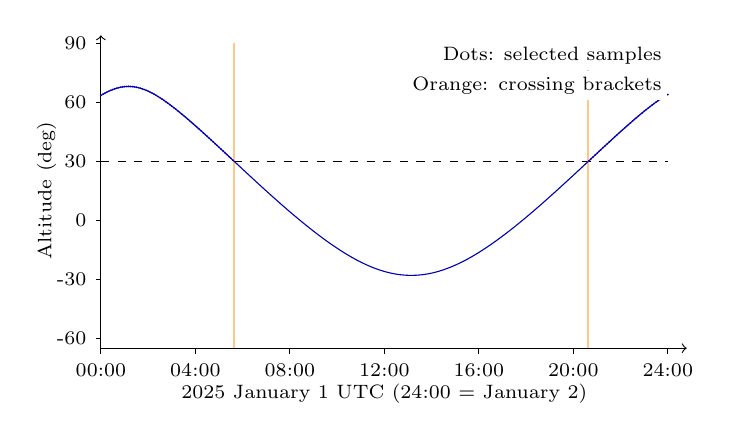
\begin{tikzpicture}[x=0.30cm,y=0.025cm,font=\scriptsize]
\draw[->] (0,-65) -- (24.8,-65);
\draw[->] (0,-65) -- (0,94);
\draw (0,-65) -- (0,-68) node[below] {00:00};
\draw (4,-65) -- (4,-68) node[below] {04:00};
\draw (8,-65) -- (8,-68) node[below] {08:00};
\draw (12,-65) -- (12,-68) node[below] {12:00};
\draw (16,-65) -- (16,-68) node[below] {16:00};
\draw (20,-65) -- (20,-68) node[below] {20:00};
\draw (24,-65) -- (24,-68) node[below] {24:00};
\draw (0,-60) -- (-0.2,-60) node[left] {-60};
\draw (0,-30) -- (-0.2,-30) node[left] {-30};
\draw (0,0) -- (-0.2,0) node[left] {0};
\draw (0,30) -- (-0.2,30) node[left] {30};
\draw (0,60) -- (-0.2,60) node[left] {60};
\draw (0,90) -- (-0.2,90) node[left] {90};
\node at (12,-88) {2025 January 1 UTC (24:00 = January 2)};
\node[rotate=90] at (-2.3,15) {Altitude (deg)};
\draw[dashed] (0,30) -- (24,30);
\fill[orange!45] (5.583333,-65) rectangle (5.666667,90);
\fill[orange!45] (20.583333,-65) rectangle (20.666667,90);
\draw[blue!70!black,thin] plot coordinates {(0.000000,63.4435271617)
(0.083333,64.0208957836)
(0.166667,64.5676418220)
(0.250000,65.0816724668)
(0.333333,65.5608515973)
(0.416667,66.0030245915)
(0.500000,66.4060497416)
(0.583333,66.7678340287)
(0.666667,67.0863744955)
(0.750000,67.3598023271)
(0.833333,67.5864294475)
(0.916667,67.7647942559)
(1.000000,67.8937045183)
(1.083333,67.9722747745)
(1.166667,67.9999551928)
(1.250000,67.9765502258)
(1.333333,67.9022252932)
(1.416667,67.7775010753)
(1.500000,67.6032359699)
(1.583333,67.3805977984)
(1.666667,67.1110271663)
(1.750000,66.7961950380)
(1.833333,66.4379567207)
(1.916667,66.0383058597)
(2.000000,65.5993293631)
(2.083333,65.1231665398)
(2.166667,64.6119719575)
(2.250000,64.0678845878)
(2.333333,63.4930015171)
(2.416667,62.8893577305)
(2.500000,62.2589110067)
(2.583333,61.6035304663)
(2.666667,60.9249902398)
(2.750000,60.2249649807)
(2.833333,59.5050294153)
(2.916667,58.7666584587)
(3.000000,58.0112303998)
(3.083333,57.2400297538)
(3.166667,56.4542518664)
(3.250000,55.6550080506)
(3.333333,54.8433299273)
(3.416667,54.0201754650)
(3.500000,53.1864332639)
(3.583333,52.3429284700)
(3.666667,51.4904267249)
(3.750000,50.6296396814)
(3.833333,49.7612285601)
(3.916667,48.8858085685)
(4.000000,48.0039530645)
(4.083333,47.1161962660)
(4.166667,46.2230374660)
(4.250000,45.3249430982)
(4.333333,44.4223504729)
(4.416667,43.5156693680)
(4.500000,42.6052853429)
(4.583333,41.6915610409)
(4.666667,40.7748385258)
(4.750000,39.8554414624)
(4.833333,38.9336759153)
(4.916667,38.0098328570)
(5.000000,37.0841885763)
(5.083333,36.1570069523)
(5.166667,35.2285396403)
(5.250000,34.2990281507)
(5.333333,33.3687039774)
(5.416667,32.4377898909)
(5.500000,31.5065011647)
(5.583333,30.5750454868)
(5.666667,29.6436246882)
(5.750000,28.7124344188)
(5.833333,27.7816657754)
(5.916667,26.8515048884)
(6.000000,25.9221344661)
(6.083333,24.9937334329)
(6.166667,24.0664777832)
(6.250000,23.1405414041)
(6.333333,22.2160956302)
(6.416667,21.2933106372)
(6.500000,20.3723548301)
(6.583333,19.4533961929)
(6.666667,18.5366016441)
(6.750000,17.6221383491)
(6.833333,16.7101731727)
(6.916667,15.8008733490)
(7.000000,14.8944071351)
(7.083333,13.9909432366)
(7.166667,13.0906520487)
(7.250000,12.1937049479)
(7.333333,11.3002755098)
(7.416667,10.4105387931)
(7.500000,9.5246725362)
(7.583333,8.6428565544)
(7.666667,7.7652733273)
(7.750000,6.8921085714)
(7.833333,6.0235506347)
(7.916667,5.1597916457)
(8.000000,4.3010267884)
(8.083333,3.4474554314)
(8.166667,2.5992804039)
(8.250000,1.7567091034)
(8.333333,0.9199528843)
(8.416667,0.0892275835)
(8.500000,-0.7352459745)
(8.583333,-1.5532425877)
(8.666667,-2.3645316321)
(8.750000,-3.1688777875)
(8.833333,-3.9660400244)
(8.916667,-4.7557723350)
(9.000000,-5.5378227561)
(9.083333,-6.3119340052)
(9.166667,-7.0778430627)
(9.250000,-7.8352807890)
(9.333333,-8.5839725781)
(9.416667,-9.3236375011)
(9.500000,-10.0539890853)
(9.583333,-10.7747345195)
(9.666667,-11.4855754599)
(9.750000,-12.1862073066)
(9.833333,-12.8763199519)
(9.916667,-13.5555975970)
(10.000000,-14.2237186267)
(10.083333,-14.8803564220)
(10.166667,-15.5251788585)
(10.250000,-16.1578492681)
(10.333333,-16.7780260458)
(10.416667,-17.3853636735)
(10.500000,-17.9795124462)
(10.583333,-18.5601194879)
(10.666667,-19.1268289909)
(10.750000,-19.6792825410)
(10.833333,-20.2171202435)
(10.916667,-20.7399807837)
(11.000000,-21.2475027120)
(11.083333,-21.7393246469)
(11.166667,-22.2150866360)
(11.250000,-22.6744304993)
(11.333333,-23.1170012024)
(11.416667,-23.5424476244)
(11.500000,-23.9504234112)
(11.583333,-24.3405884240)
(11.666667,-24.7126093914)
(11.750000,-25.0661614482)
(11.833333,-25.4009288788)
(11.916667,-25.7166066539)
(12.000000,-26.0129012368)
(12.083333,-26.2895320492)
(12.166667,-26.5462324841)
(12.250000,-26.7827509451)
(12.333333,-26.9988521799)
(12.416667,-27.1943180835)
(12.500000,-27.3689489350)
(12.583333,-27.5225641293)
(12.666667,-27.6550032337)
(12.750000,-27.7661266091)
(12.833333,-27.8558162366)
(12.916667,-27.9239762468)
(13.000000,-27.9705333940)
(13.083333,-27.9954374902)
(13.166667,-27.9986616147)
(13.250000,-27.9802022810)
(13.333333,-27.9400794512)
(13.416667,-27.8783364128)
(13.500000,-27.7950395967)
(13.583333,-27.6902781846)
(13.666667,-27.5641636642)
(13.750000,-27.4168293287)
(13.833333,-27.2484294849)
(13.916667,-27.0591388513)
(14.000000,-26.8491515323)
(14.083333,-26.6186802999)
(14.166667,-26.3679553814)
(14.250000,-26.0972236642)
(14.333333,-25.8067473794)
(14.416667,-25.4968030680)
(14.500000,-25.1676805714)
(14.583333,-24.8196815731)
(14.666667,-24.4531187859)
(14.750000,-24.0683144183)
(14.833333,-23.6655994194)
(14.916667,-23.2453119394)
(15.000000,-22.8077966611)
(15.083333,-22.3534033460)
(15.166667,-21.8824859662)
(15.250000,-21.3954019208)
(15.333333,-20.8925106526)
(15.416667,-20.3741732843)
(15.500000,-19.8407512467)
(15.583333,-19.2926060544)
(15.666667,-18.7300980092)
(15.750000,-18.1535861187)
(15.833333,-17.5634269580)
(15.916667,-16.9599743270)
(16.000000,-16.3435789939)
(16.083333,-15.7145876679)
(16.166667,-15.0733432546)
(16.250000,-14.4201838224)
(16.333333,-13.7554429783)
(16.416667,-13.0794488981)
(16.500000,-12.3925248115)
(16.583333,-11.6949881827)
(16.666667,-10.9871508231)
(16.750000,-10.2693190645)
(16.833333,-9.5417930036)
(16.916667,-8.8048672155)
(17.000000,-8.0588299420)
(17.083333,-7.3039638768)
(17.166667,-6.5405453830)
(17.250000,-5.7688453406)
(17.333333,-4.9891284902)
(17.416667,-4.2016538102)
(17.500000,-3.4066749286)
(17.583333,-2.6044394860)
(17.666667,-1.7951901061)
(17.750000,-0.9791636638)
(17.833333,-0.1565922937)
(17.916667,0.6722973371)
(18.000000,1.5072829878)
(18.083333,2.3481474557)
(18.166667,3.1946780727)
(18.250000,4.0466661828)
(18.333333,4.9039077537)
(18.416667,5.7662022718)
(18.500000,6.6333534668)
(18.583333,7.5051681854)
(18.666667,8.3814571158)
(18.750000,9.2620336423)
(18.833333,10.1467144504)
(18.916667,11.0353189566)
(19.000000,11.9276687229)
(19.083333,12.8235880603)
(19.166667,13.7229028351)
(19.250000,14.6254411860)
(19.333333,15.5310323093)
(19.416667,16.4395071686)
(19.500000,17.3506972578)
(19.583333,18.2644351767)
(19.666667,19.1805539820)
(19.750000,20.0988865201)
(19.833333,21.0192659789)
(19.916667,21.9415245797)
(20.000000,22.8654942264)
(20.083333,23.7910051615)
(20.166667,24.7178865833)
(20.250000,25.6459652591)
(20.333333,26.5750659779)
(20.416667,27.5050107353)
(20.500000,28.4356178888)
(20.583333,29.3667025295)
(20.666667,30.2980749482)
(20.750000,31.2295410608)
(20.833333,32.1609007943)
(20.916667,33.0919484245)
(21.000000,34.0224708642)
(21.083333,34.9522477695)
(21.166667,35.8810503332)
(21.250000,36.8086400129)
(21.333333,37.7347684271)
(21.416667,38.6591753025)
(21.500000,39.5815883170)
(21.583333,40.5017208575)
(21.666667,41.4192716475)
(21.750000,42.3339222756)
(21.833333,43.2453364411)
(21.916667,44.1531578180)
(22.000000,45.0570077691)
(22.083333,45.9564840983)
(22.166667,46.8511577953)
(22.250000,47.7405715094)
(22.333333,48.6242358801)
(22.416667,49.5016275458)
(22.500000,50.3721850036)
(22.583333,51.2353059801)
(22.666667,52.0903433500)
(22.750000,52.9366007967)
(22.833333,53.7733293388)
(22.916667,54.5997218855)
(23.000000,55.4149093561)
(23.083333,56.2179548120)
(23.166667,57.0078492048)
(23.250000,57.7835053290)
(23.333333,58.5437534397)
(23.416667,59.2873360127)
(23.500000,60.0129029646)
(23.583333,60.7190085406)
(23.666667,61.4041077478)
(23.750000,62.0665557374)
(23.833333,62.7046075846)
(23.916667,63.3164219447)
(24.000000,63.9000663521)};
\fill[blue!70!black] (0.000000,63.4435271617) circle[radius=0.35pt];
\fill[blue!70!black] (0.083333,64.0208957836) circle[radius=0.35pt];
\fill[blue!70!black] (0.166667,64.5676418220) circle[radius=0.35pt];
\fill[blue!70!black] (0.250000,65.0816724668) circle[radius=0.35pt];
\fill[blue!70!black] (0.333333,65.5608515973) circle[radius=0.35pt];
\fill[blue!70!black] (0.416667,66.0030245915) circle[radius=0.35pt];
\fill[blue!70!black] (0.500000,66.4060497416) circle[radius=0.35pt];
\fill[blue!70!black] (0.583333,66.7678340287) circle[radius=0.35pt];
\fill[blue!70!black] (0.666667,67.0863744955) circle[radius=0.35pt];
\fill[blue!70!black] (0.750000,67.3598023271) circle[radius=0.35pt];
\fill[blue!70!black] (0.833333,67.5864294475) circle[radius=0.35pt];
\fill[blue!70!black] (0.916667,67.7647942559) circle[radius=0.35pt];
\fill[blue!70!black] (1.000000,67.8937045183) circle[radius=0.35pt];
\fill[blue!70!black] (1.083333,67.9722747745) circle[radius=0.35pt];
\fill[blue!70!black] (1.166667,67.9999551928) circle[radius=0.35pt];
\fill[blue!70!black] (1.250000,67.9765502258) circle[radius=0.35pt];
\fill[blue!70!black] (1.333333,67.9022252932) circle[radius=0.35pt];
\fill[blue!70!black] (1.416667,67.7775010753) circle[radius=0.35pt];
\fill[blue!70!black] (1.500000,67.6032359699) circle[radius=0.35pt];
\fill[blue!70!black] (1.583333,67.3805977984) circle[radius=0.35pt];
\fill[blue!70!black] (1.666667,67.1110271663) circle[radius=0.35pt];
\fill[blue!70!black] (1.750000,66.7961950380) circle[radius=0.35pt];
\fill[blue!70!black] (1.833333,66.4379567207) circle[radius=0.35pt];
\fill[blue!70!black] (1.916667,66.0383058597) circle[radius=0.35pt];
\fill[blue!70!black] (2.000000,65.5993293631) circle[radius=0.35pt];
\fill[blue!70!black] (2.083333,65.1231665398) circle[radius=0.35pt];
\fill[blue!70!black] (2.166667,64.6119719575) circle[radius=0.35pt];
\fill[blue!70!black] (2.250000,64.0678845878) circle[radius=0.35pt];
\fill[blue!70!black] (2.333333,63.4930015171) circle[radius=0.35pt];
\fill[blue!70!black] (2.416667,62.8893577305) circle[radius=0.35pt];
\fill[blue!70!black] (2.500000,62.2589110067) circle[radius=0.35pt];
\fill[blue!70!black] (2.583333,61.6035304663) circle[radius=0.35pt];
\fill[blue!70!black] (2.666667,60.9249902398) circle[radius=0.35pt];
\fill[blue!70!black] (2.750000,60.2249649807) circle[radius=0.35pt];
\fill[blue!70!black] (2.833333,59.5050294153) circle[radius=0.35pt];
\fill[blue!70!black] (2.916667,58.7666584587) circle[radius=0.35pt];
\fill[blue!70!black] (3.000000,58.0112303998) circle[radius=0.35pt];
\fill[blue!70!black] (3.083333,57.2400297538) circle[radius=0.35pt];
\fill[blue!70!black] (3.166667,56.4542518664) circle[radius=0.35pt];
\fill[blue!70!black] (3.250000,55.6550080506) circle[radius=0.35pt];
\fill[blue!70!black] (3.333333,54.8433299273) circle[radius=0.35pt];
\fill[blue!70!black] (3.416667,54.0201754650) circle[radius=0.35pt];
\fill[blue!70!black] (3.500000,53.1864332639) circle[radius=0.35pt];
\fill[blue!70!black] (3.583333,52.3429284700) circle[radius=0.35pt];
\fill[blue!70!black] (3.666667,51.4904267249) circle[radius=0.35pt];
\fill[blue!70!black] (3.750000,50.6296396814) circle[radius=0.35pt];
\fill[blue!70!black] (3.833333,49.7612285601) circle[radius=0.35pt];
\fill[blue!70!black] (3.916667,48.8858085685) circle[radius=0.35pt];
\fill[blue!70!black] (4.000000,48.0039530645) circle[radius=0.35pt];
\fill[blue!70!black] (4.083333,47.1161962660) circle[radius=0.35pt];
\fill[blue!70!black] (4.166667,46.2230374660) circle[radius=0.35pt];
\fill[blue!70!black] (4.250000,45.3249430982) circle[radius=0.35pt];
\fill[blue!70!black] (4.333333,44.4223504729) circle[radius=0.35pt];
\fill[blue!70!black] (4.416667,43.5156693680) circle[radius=0.35pt];
\fill[blue!70!black] (4.500000,42.6052853429) circle[radius=0.35pt];
\fill[blue!70!black] (4.583333,41.6915610409) circle[radius=0.35pt];
\fill[blue!70!black] (4.666667,40.7748385258) circle[radius=0.35pt];
\fill[blue!70!black] (4.750000,39.8554414624) circle[radius=0.35pt];
\fill[blue!70!black] (4.833333,38.9336759153) circle[radius=0.35pt];
\fill[blue!70!black] (4.916667,38.0098328570) circle[radius=0.35pt];
\fill[blue!70!black] (5.000000,37.0841885763) circle[radius=0.35pt];
\fill[blue!70!black] (5.083333,36.1570069523) circle[radius=0.35pt];
\fill[blue!70!black] (5.166667,35.2285396403) circle[radius=0.35pt];
\fill[blue!70!black] (5.250000,34.2990281507) circle[radius=0.35pt];
\fill[blue!70!black] (5.333333,33.3687039774) circle[radius=0.35pt];
\fill[blue!70!black] (5.416667,32.4377898909) circle[radius=0.35pt];
\fill[blue!70!black] (5.500000,31.5065011647) circle[radius=0.35pt];
\fill[blue!70!black] (5.583333,30.5750454868) circle[radius=0.35pt];
\fill[blue!70!black] (20.666667,30.2980749482) circle[radius=0.35pt];
\fill[blue!70!black] (20.750000,31.2295410608) circle[radius=0.35pt];
\fill[blue!70!black] (20.833333,32.1609007943) circle[radius=0.35pt];
\fill[blue!70!black] (20.916667,33.0919484245) circle[radius=0.35pt];
\fill[blue!70!black] (21.000000,34.0224708642) circle[radius=0.35pt];
\fill[blue!70!black] (21.083333,34.9522477695) circle[radius=0.35pt];
\fill[blue!70!black] (21.166667,35.8810503332) circle[radius=0.35pt];
\fill[blue!70!black] (21.250000,36.8086400129) circle[radius=0.35pt];
\fill[blue!70!black] (21.333333,37.7347684271) circle[radius=0.35pt];
\fill[blue!70!black] (21.416667,38.6591753025) circle[radius=0.35pt];
\fill[blue!70!black] (21.500000,39.5815883170) circle[radius=0.35pt];
\fill[blue!70!black] (21.583333,40.5017208575) circle[radius=0.35pt];
\fill[blue!70!black] (21.666667,41.4192716475) circle[radius=0.35pt];
\fill[blue!70!black] (21.750000,42.3339222756) circle[radius=0.35pt];
\fill[blue!70!black] (21.833333,43.2453364411) circle[radius=0.35pt];
\fill[blue!70!black] (21.916667,44.1531578180) circle[radius=0.35pt];
\fill[blue!70!black] (22.000000,45.0570077691) circle[radius=0.35pt];
\fill[blue!70!black] (22.083333,45.9564840983) circle[radius=0.35pt];
\fill[blue!70!black] (22.166667,46.8511577953) circle[radius=0.35pt];
\fill[blue!70!black] (22.250000,47.7405715094) circle[radius=0.35pt];
\fill[blue!70!black] (22.333333,48.6242358801) circle[radius=0.35pt];
\fill[blue!70!black] (22.416667,49.5016275458) circle[radius=0.35pt];
\fill[blue!70!black] (22.500000,50.3721850036) circle[radius=0.35pt];
\fill[blue!70!black] (22.583333,51.2353059801) circle[radius=0.35pt];
\fill[blue!70!black] (22.666667,52.0903433500) circle[radius=0.35pt];
\fill[blue!70!black] (22.750000,52.9366007967) circle[radius=0.35pt];
\fill[blue!70!black] (22.833333,53.7733293388) circle[radius=0.35pt];
\fill[blue!70!black] (22.916667,54.5997218855) circle[radius=0.35pt];
\fill[blue!70!black] (23.000000,55.4149093561) circle[radius=0.35pt];
\fill[blue!70!black] (23.083333,56.2179548120) circle[radius=0.35pt];
\fill[blue!70!black] (23.166667,57.0078492048) circle[radius=0.35pt];
\fill[blue!70!black] (23.250000,57.7835053290) circle[radius=0.35pt];
\fill[blue!70!black] (23.333333,58.5437534397) circle[radius=0.35pt];
\fill[blue!70!black] (23.416667,59.2873360127) circle[radius=0.35pt];
\fill[blue!70!black] (23.500000,60.0129029646) circle[radius=0.35pt];
\fill[blue!70!black] (23.583333,60.7190085406) circle[radius=0.35pt];
\fill[blue!70!black] (23.666667,61.4041077478) circle[radius=0.35pt];
\fill[blue!70!black] (23.750000,62.0665557374) circle[radius=0.35pt];
\fill[blue!70!black] (23.833333,62.7046075846) circle[radius=0.35pt];
\fill[blue!70!black] (23.916667,63.3164219447) circle[radius=0.35pt];
\fill[blue!70!black] (24.000000,63.9000663521) circle[radius=0.35pt];
\node[anchor=north east,fill=white,inner sep=2pt] at (24,91) {Dots: selected samples};
\node[anchor=north east,fill=white,inner sep=2pt] at (24,76) {Orange: crossing brackets};
\end{tikzpicture}

\caption{All 289 terrestrial altitude samples. The line joins sampled values;
dots mark the 109 selected samples, and the dashed line is the $30^\circ$
threshold. Shaded five-minute brackets contain the two crossings; no refined
event times are implied. The plot is based on the 289 evaluated samples;
its plotting code was AI-assisted.}
\label{fig:viewing-window}
\end{figure}

\subsection{Earth seen from a lunar surface site}
\label{sec:lunar-example}

Our second application computes Earth's geometric altitude, azimuth and range
from a lunar station at $20^\circ$ east longitude and $-3.5^\circ$
planetocentric latitude at TT JD $2460000.5$. The observer lies on the
$1737.4$ km reference sphere, so the local vertical is radial. This calculation
combines a finite-distance ephemeris target with the generic surface-observer
architecture introduced in Siderust v0.16.0.

Listing~\ref{lst:moon-surface} loads the DE440s kernel and evaluates the Moon's
geocentric position. Reversing that vector gives Earth's selenocentric position
in the same mean-ecliptic J2000 frame. The explicit \texttt{EarthFromMoon}
alias retains the target's center, frame and length unit. The surface API
rotates the target into the lunar body-fixed frame, subtracts the observer
position and projects the resulting line of sight onto the local horizon.
The target remains a position throughout, preserving range and parallax.
Writing $\boldsymbol r$ for Earth's selenocentric inertial vector,
$R$ for the inertial-to-body-fixed rotation, and $\boldsymbol s$ for the
body-fixed site, the local vector is
\begin{equation}
 \boldsymbol\ell =
 \begin{pmatrix}\boldsymbol n^{\mathsf T}\\
                 \boldsymbol e^{\mathsf T}\\
                 \boldsymbol u^{\mathsf T}\end{pmatrix}
 (R\boldsymbol r-\boldsymbol s),
\end{equation}
where $\boldsymbol n$, $\boldsymbol e$ and $\boldsymbol u$ are the local
north, east and up unit vectors. Range is $\lVert\boldsymbol\ell\rVert$;
altitude is $\operatorname{atan2}(\ell_u,\sqrt{\ell_n^2+\ell_e^2})$
and azimuth is $\operatorname{atan2}(\ell_e,\ell_n)$ modulo $2\pi$.
This ordering makes the observer subtraction and azimuth signs explicit.

\lstinputlisting[float=tbp,caption={Earth from a lunar observer using published v0.16.0 APIs. The argument supplies the DE440s BSP file. The output is altitude and azimuth in degrees, followed by range in kilometres.},label={lst:moon-surface}]{../examples/src/bin/earth_from_moon.rs}

The result is altitude $\EarthAltitude^\circ$, azimuth $\EarthAzimuth^\circ$ and range
$\EarthRange$ km. An independent CSPICE reduction of the same ephemeris and
surface geometry agrees within $\EarthAngleBound$ degrees and
$\EarthRangeBound$ km. The corresponding Moon-center direction has altitude
$\CentreAltitude^\circ$: observer displacement changes the altitude by about
$\EarthParallax^\circ$. This difference demonstrates why a nearby target requires
finite-distance geometry. The selected Earth position is above the horizon;
the example computes a pointing state rather than an Earthrise event.

We use the analytical text-PCK \texttt{IAU\_MOON} orientation,
which approximates the lunar mean-Earth/polar-axis convention and is exposed as \texttt{MoonIauMeanEarth}. Its periodic arguments use
TDB converted from the supplied TT epoch. This model is distinct from
DE-specific \texttt{MOON\_PA} and binary-PCK \texttt{MOON\_ME} realizations
\cite{archinal2011,naiflunarframes}. Azimuth increases from north through east.
Both applications compute geometric quantities, with atmospheric refraction,
light time, aberration, deflection and terrain masking omitted. These model
choices define the observables used in the comparisons.
